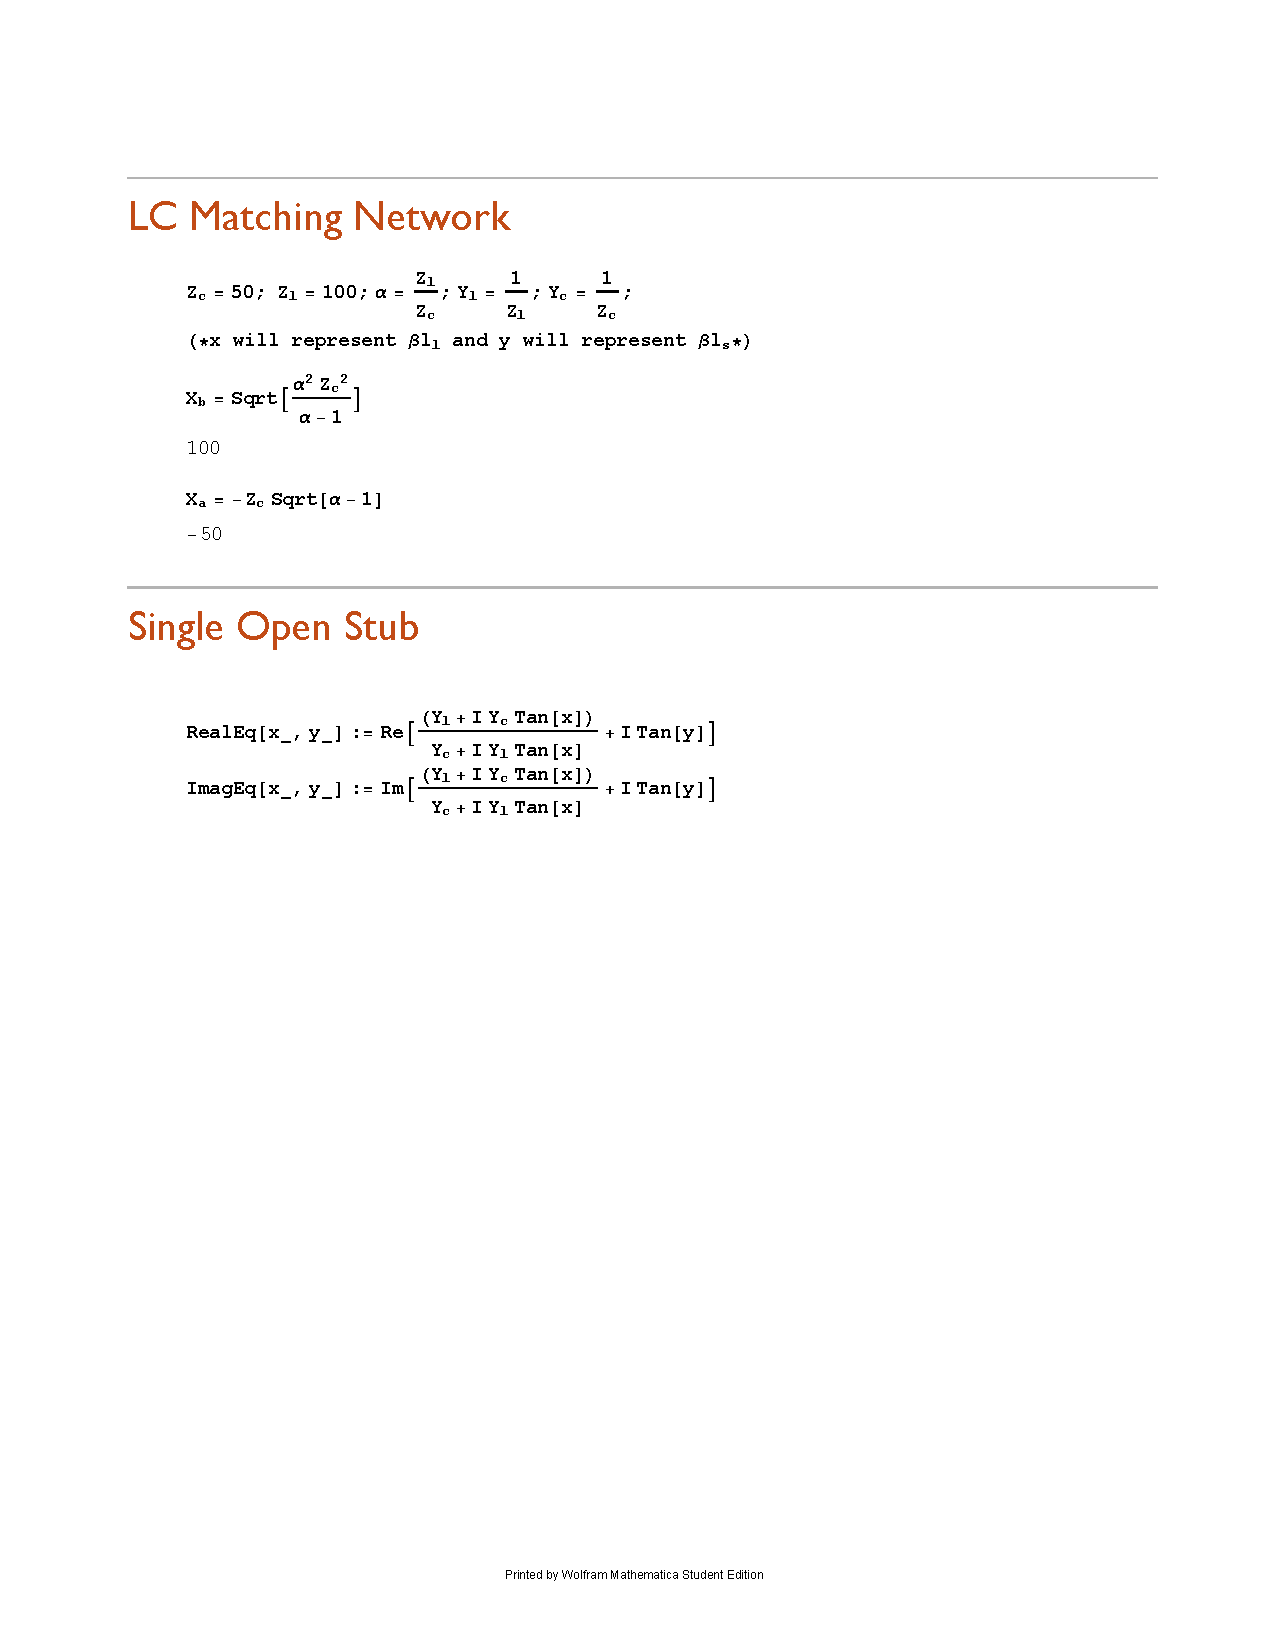
\includepdf[pagecommand={\section{Problem 2 Appendix}\subsection{Mathematica}},scale=.9,pages=1,clip,trim=0cm 5cm 0cm
0cm]{res/Mathematica/Problem2.pdf}
\includepdf[scale=.9,pages=2-,clip,trim=2cm 5cm 0cm 2cm]{res/Mathematica/Problem2.pdf}
\includepdf[scale=.9,pages=2-,clip,trim=2cm 5cm 0cm 2cm]{res/Mathematica/Problem2.pdf}

\begin{figure}[h]
    \centering
    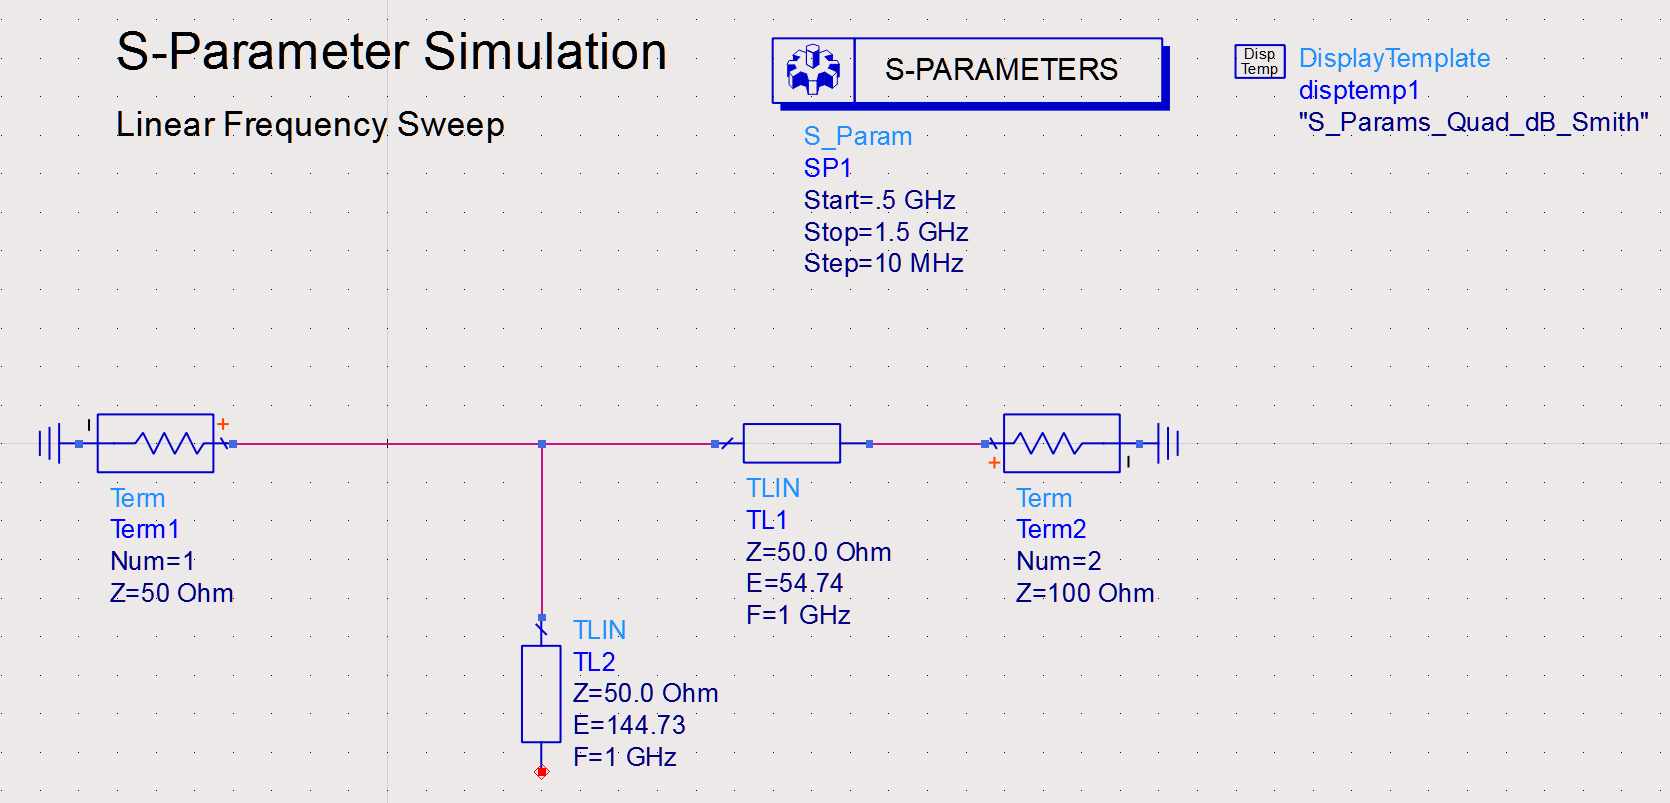
\includegraphics[width=0.8\linewidth]{res/ADS/SingleOpenStubSchematic.png}
    \caption{Schematic for the single open stub tuner.}
    \label{fig:}
\end{figure}
\begin{figure}[h]
    \centering
    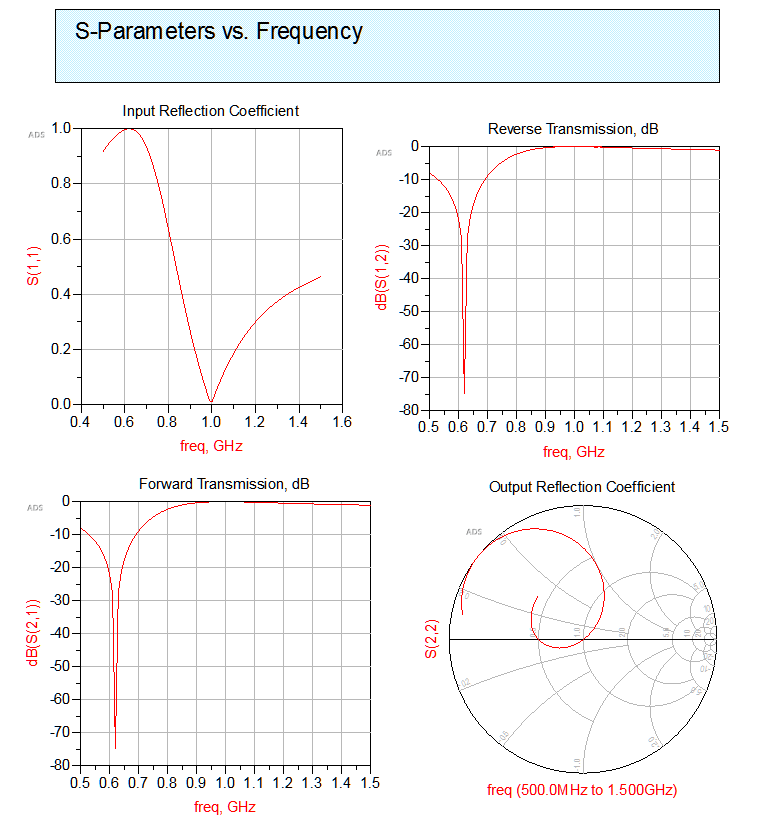
\includegraphics[width=0.8\linewidth]{res/ADS/SingleOpenStub.png}
    \caption{Results for the single open stub tuner.}
    \label{fig:}
\end{figure}

\begin{figure}[h]
    \centering
    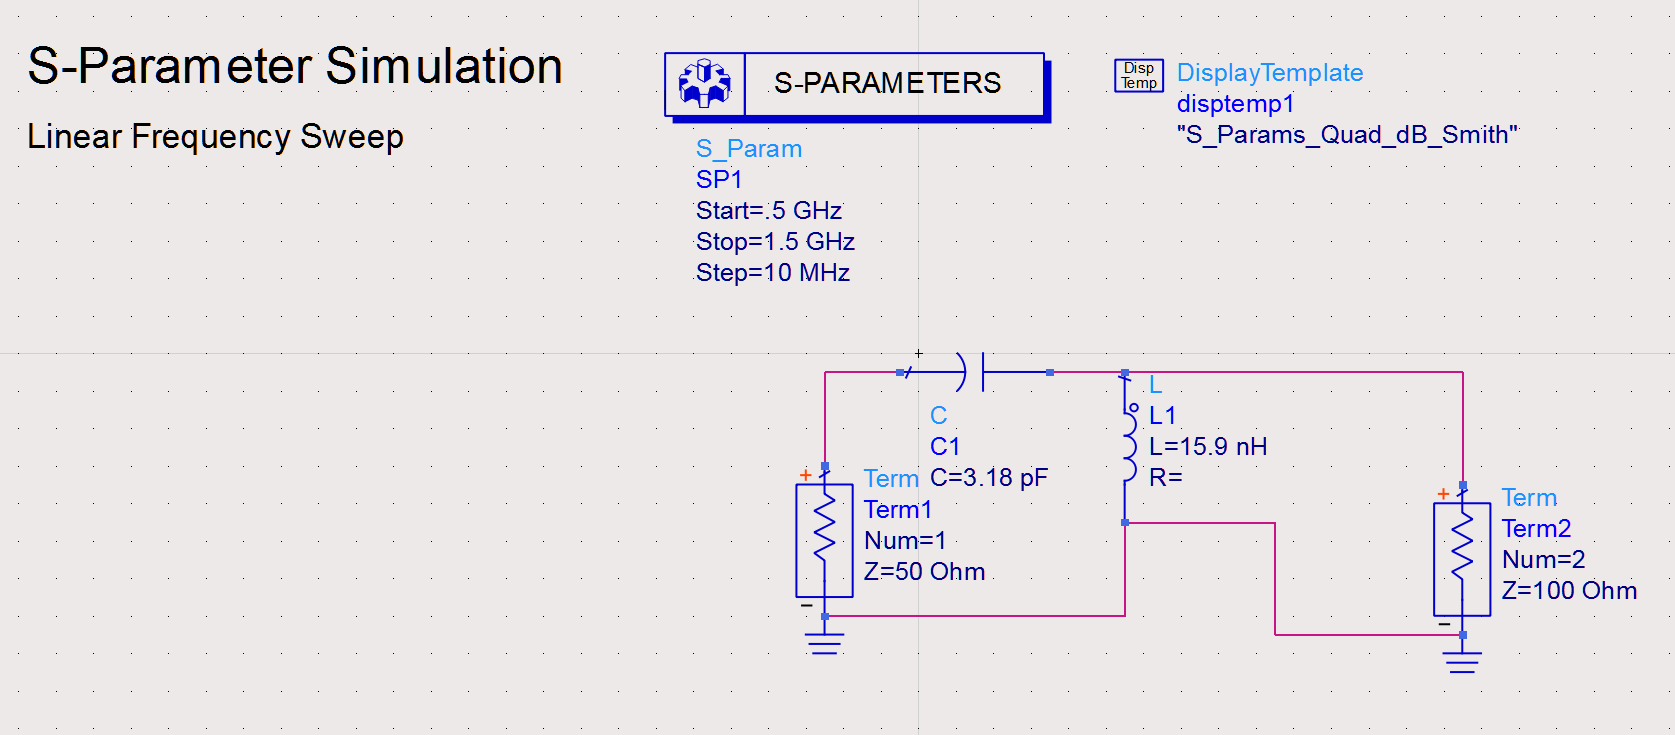
\includegraphics[width=0.8\linewidth]{res/ADS/LCMatchingNetworkSchematic.png}
    \caption{Schematic for the LC Matching Network.}
    \label{fig:}
\end{figure}
\begin{figure}[h]
    \centering
    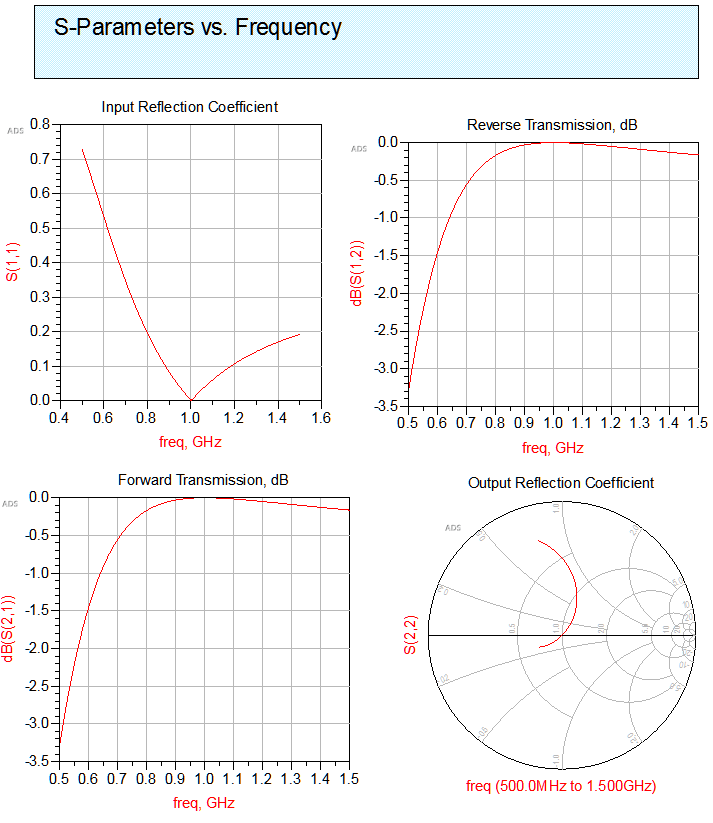
\includegraphics[width=0.8\linewidth]{res/ADS/LCMatchingNetwork.png}
    \caption{Results for the LC Matching Network.}
    \label{fig:}
\end{figure}

\begin{figure}[h]
    \centering
    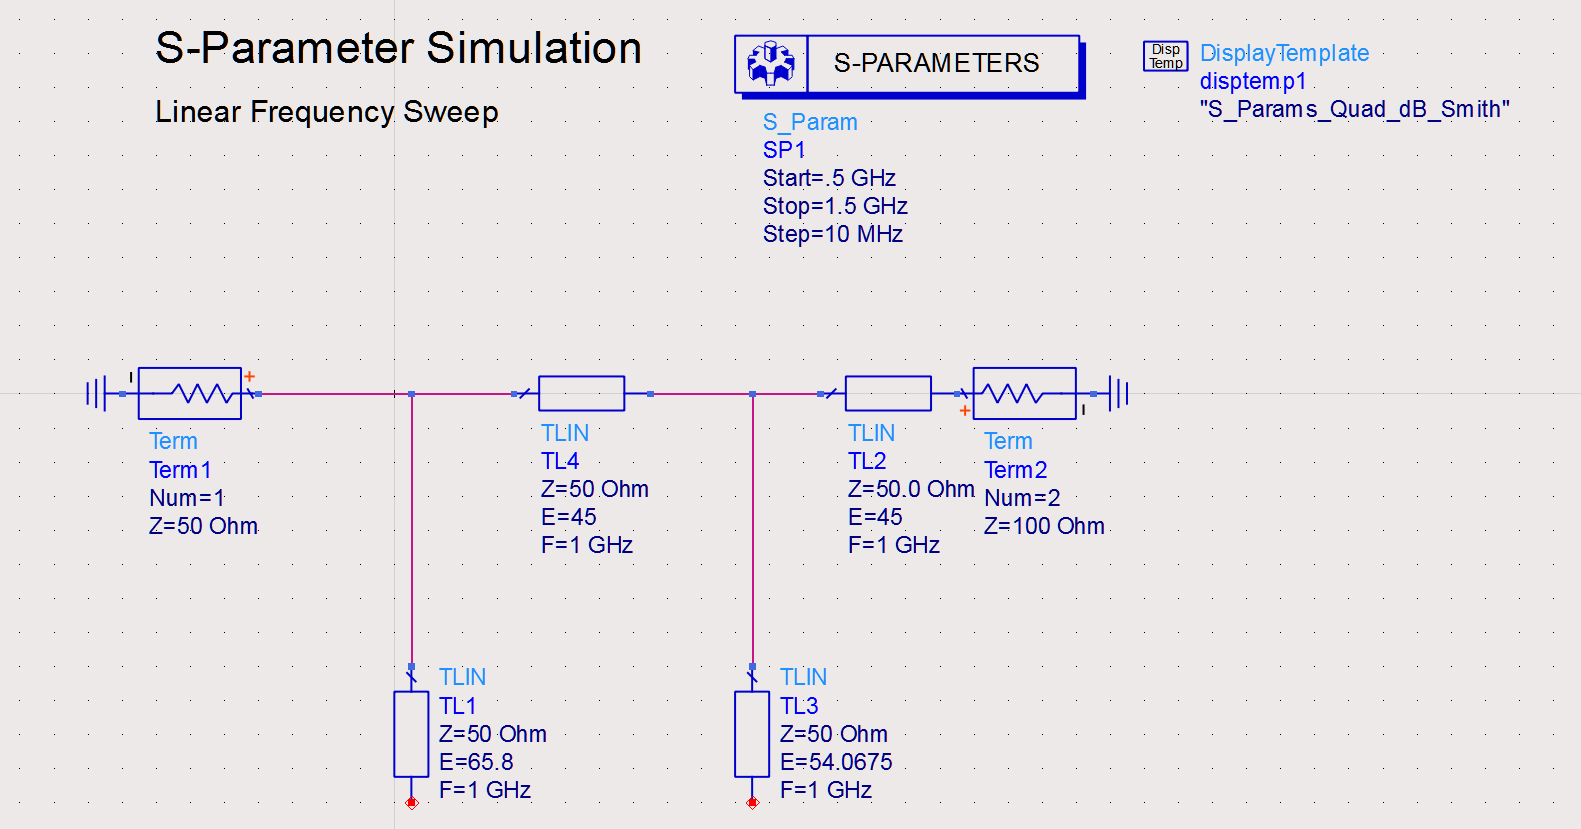
\includegraphics[width=0.8\linewidth]{res/ADS/DoubleOpenStubSchematic.png}
    \caption{Schematic for the double open stub tuner.}
    \label{fig:}
\end{figure}
\begin{figure}[h]
    \centering
    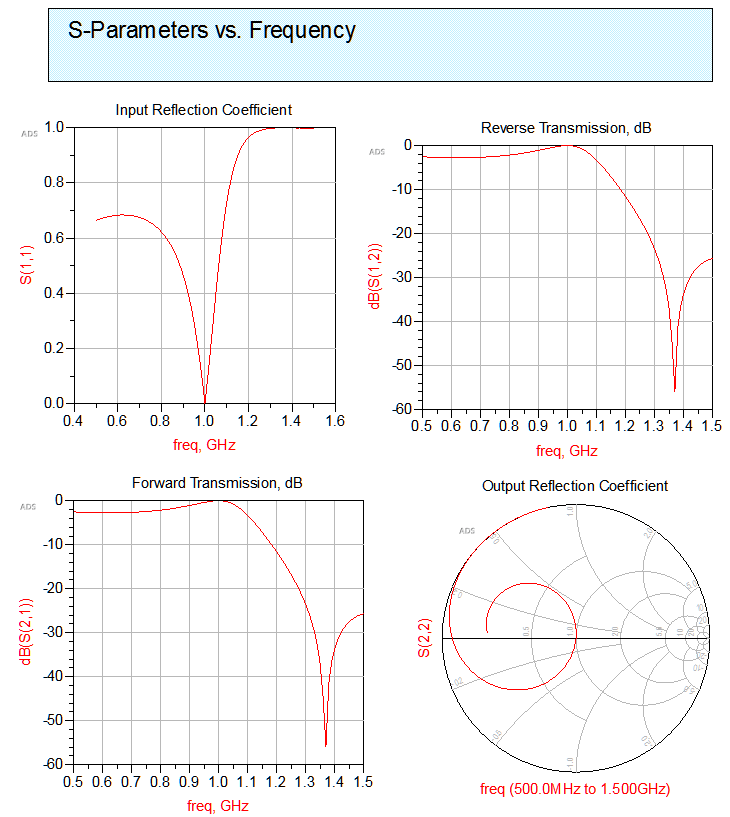
\includegraphics[width=0.8\linewidth]{res/ADS/DoubleOpenStub.png}
    \caption{Results for the double open stub tuner.}
    \label{fig:}
\end{figure}
